\pdfoutput=1
\documentclass[11pt]{article}
\usepackage{amsmath}
\usepackage{amsfonts}
\usepackage{amssymb}
\usepackage[]{NLPAICS2024}
\usepackage{times}
\usepackage{latexsym}
\usepackage[T1]{fontenc}
\usepackage[utf8]{inputenc}
\usepackage{microtype}
\usepackage{inconsolata}
\usepackage{graphicx}
\usepackage{listings}
\usepackage{minted} 
\usepackage{booktabs} % Required for better table lines

\title{NLP: Text Generation \\
Story Continuation}

\author{Kavyanjali Agnihotri \\ Matriculation Number: 6975801}

\begin{document}

\maketitle

\section{Introduction}
This report explores the task of story continuation using two transformer-based models (BART and T5). The goal is to generate coherent and contextually appropriate continuations for given story prompts. We analyze the dataset, preprocess it for topic modeling (LDA), and evaluate zero-shot vs. fine-tuned performance of BART and T5.

\section{Dataset}
We chose the dataset as \texttt{WritingPrompts} from hugging face. The dataset consists of short story prompts and their continuations (story). It was split into 'train', 'test' and 'validation' sets. The total entries in the dataset were 303,358 that were prompt-story pairs. 

An example entry is as follows: 
\begin{verbatim}
{'prompt': "[ WP ] You 've finally managed 
to discover the secret ... you . ''\n",
 'story': "So many times have I walked on 
 ... death, is inescapable.\n"}
\end{verbatim}

\subsection{General Preprocessing and Cleaning}
The dataset was preprocessed and cleaned by removing special and rare characters, and all text was converted to lowercase. Additionally, entries containing prompts with fewer than 10 words were excluded, as were stories with fewer than 150 words. This filtering ensured that zero-shot models received sufficiently informative prompts for story generation, while fine-tuned models were provided with adequate context for coherent story progression. After this, the dataset had 264,949 entries. 

\subsection{Initial Analysis}
The main statistics of the dataset are as:
\begin{itemize}
    \item Average words per prompt: 28.4
    \item Average words per story: 553.2
    \item Ratio of story words to prompt words: 19.5
\end{itemize}

Notable observations include the presence of \texttt{'\textbackslash n'} in the stories, which plays a crucial role in maintaining dialogue structure and narrative flow for model generation. Additionally, prompts are typically prefixed with the token \texttt{'[WP]'}. Some prompts, however, consist of only a single word, which could impact the model's ability to generate coherent and contextually rich narratives so we some entries removed as described above.


\section{Latent Dirichlet Allocation (LDA)}
Latent Dirichlet Allocation (LDA) is a generative probabilistic model commonly used for topic modeling in natural language processing. It operates under the assumption that documents are mixtures of latent topics, where each topic is characterized by a distribution over words. LDA employs a Bayesian framework utilizing priors to model document-topic and topic-word distributions. This results in the discovery of underlying thematic structures in unstructured text corpora. This unsupervised learning technique is useful for tasks such as document clustering, summarization, and feature extraction in text analysis. 

We applied LDA to the \texttt{WritingPrompts} dataset which contains paired prompts and stories to identify the top five recurring themes or topics. This analysis helps uncover dominant narrative patterns, providing insights into the dataset’s inherent structure.


\subsection{Preprocessing for LDA}
Before applying LDA, the text data underwent several preprocessing steps to improve topic modeling quality:

\begin{itemize}
    \item \textbf{Tokenization}: Text was split into individual words using \texttt{nltk.word\_tokenize}, converting raw text into analyzable units
    
    \item \textbf{Stopword Removal}: Common uninformative words (e.g., "the", "and") were removed using \texttt{nltk.corpus.stopwords} to reduce noise and focus on meaningful terms
    
    \item \textbf{Lemmatization}: Words were reduced to their base forms (e.g., "running" $\rightarrow$ "run") using \texttt{WordNetLemmatizer} to treat morphological variations as single features
\end{itemize}

For topic modeling, the \textit{prompt} and \textit{story} columns were concatenated into a \texttt{full\_text} field to preserve narrative context. The text corpus was further refined by filtering which retained terms appearing in $\geq$15 documents while excluding those in $>$50\% of documents to balance topic.

\subsection{Training LDA Model}
The LDA model was trained using \texttt{gensim.models.LdaModel} with the following configuration:

\begin{verbatim}
LdaModel(corpus=corpus,
    id2word=dictionary,
    num_topics=num_topics,
    random_state=42,
    update_every=1,
    chunksize=100,
    passes=10,
    alpha='auto',
    per_word_topics=True)
\end{verbatim}

Key parameters of training included:
\begin{itemize}
    \item Number of latent topics to discover = \texttt{5}
    \item Training \texttt{10} iterations through the corpus
    \item Ensures reproducibility by \texttt{random\_state=42}
\end{itemize}

\subsection{LDA Results and Analysis}
The model identified the following thematic patterns:

\begin{itemize}
    \item \textbf{Topic 0 (Dialogue / Physical Interaction)}: 
        Character-driven scenes with conversations and physical descriptions
    \item \textbf{Topic 1 (Existential/Worldly Reflection)}: 
        Philosophical themes about mortality and spirituality
    \item \textbf{Topic 2 (Sci-Fi/Exploration)}: 
        Futuristic narratives involving space and alien encounters
    \item \textbf{Topic 3 (Casual Reflection)}: 
        Everyday conversations and internal monologues
    \item \textbf{Topic 4 (Sensory/Environment)}: 
        Descriptive passages focusing on physical surroundings
\end{itemize}

A training document showed this topic distribution as \texttt{Topic 0: 0.328}, \texttt{Topic 1: 0.204}, \texttt{Topic 2: 0.032}, \texttt{Topic 3: 0.161} and \texttt{Topic 4: 0.275}. The document's content is primarily dialogue-driven, accounting for 32.8\% (Topic 0) and exhibits a strong environmental context at 27.5\% (Topic 4). Secondary themes include existential elements which makes up 20.4\% (Topic 1). With only a minimal presence of sci-fi elements (3.2\% Topic 2) implying the document leans towards realistic fiction.

\begin{figure}[htbp]
    \centering
    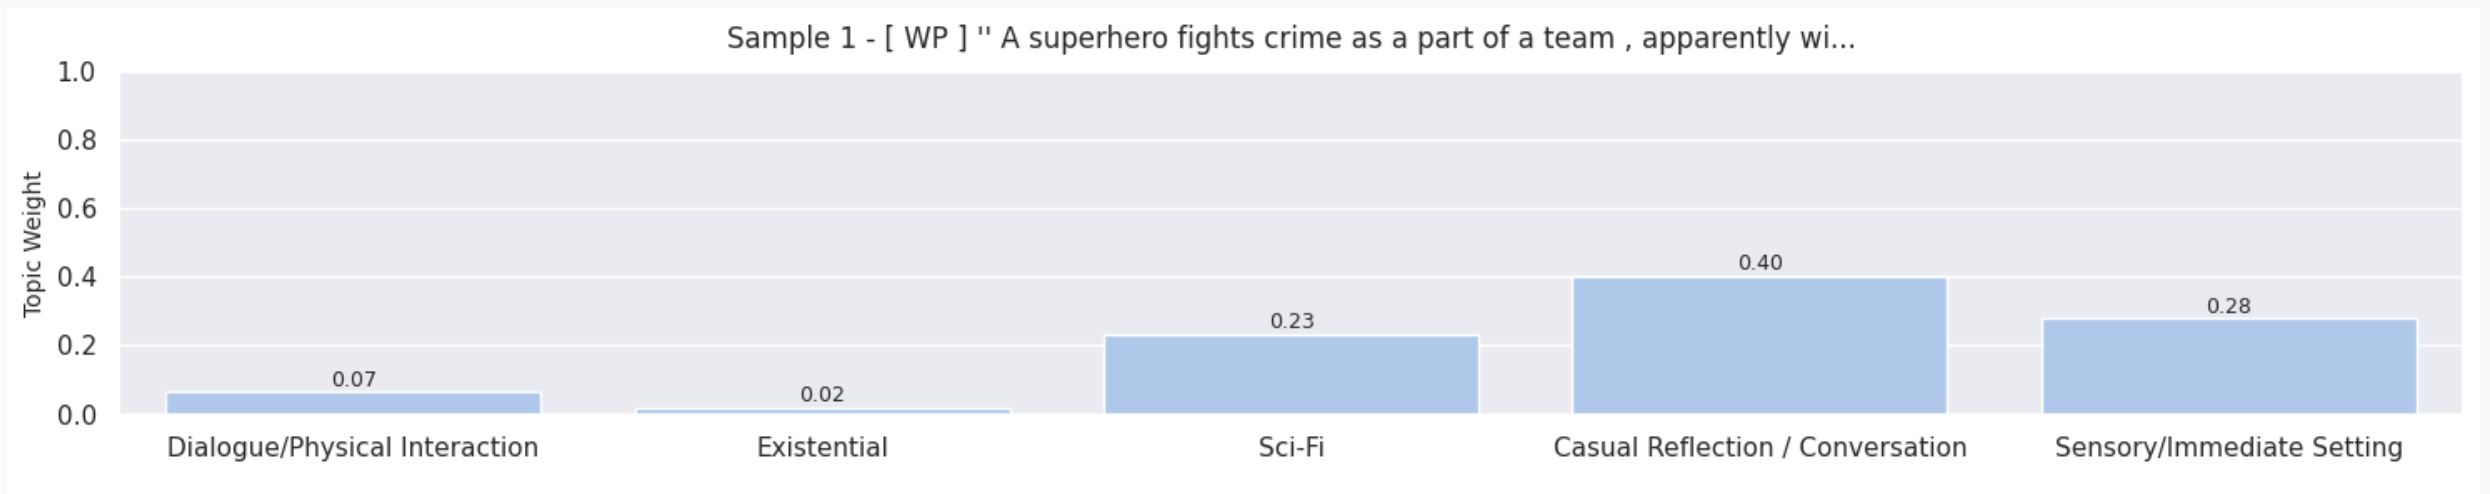
\includegraphics[width=0.5\textwidth]{lda1.png}
    \caption{Plot showing the topic distribution of the given prompt}
    \label{fig:lda1}
\end{figure}

\begin{figure}[htbp]
    \centering
    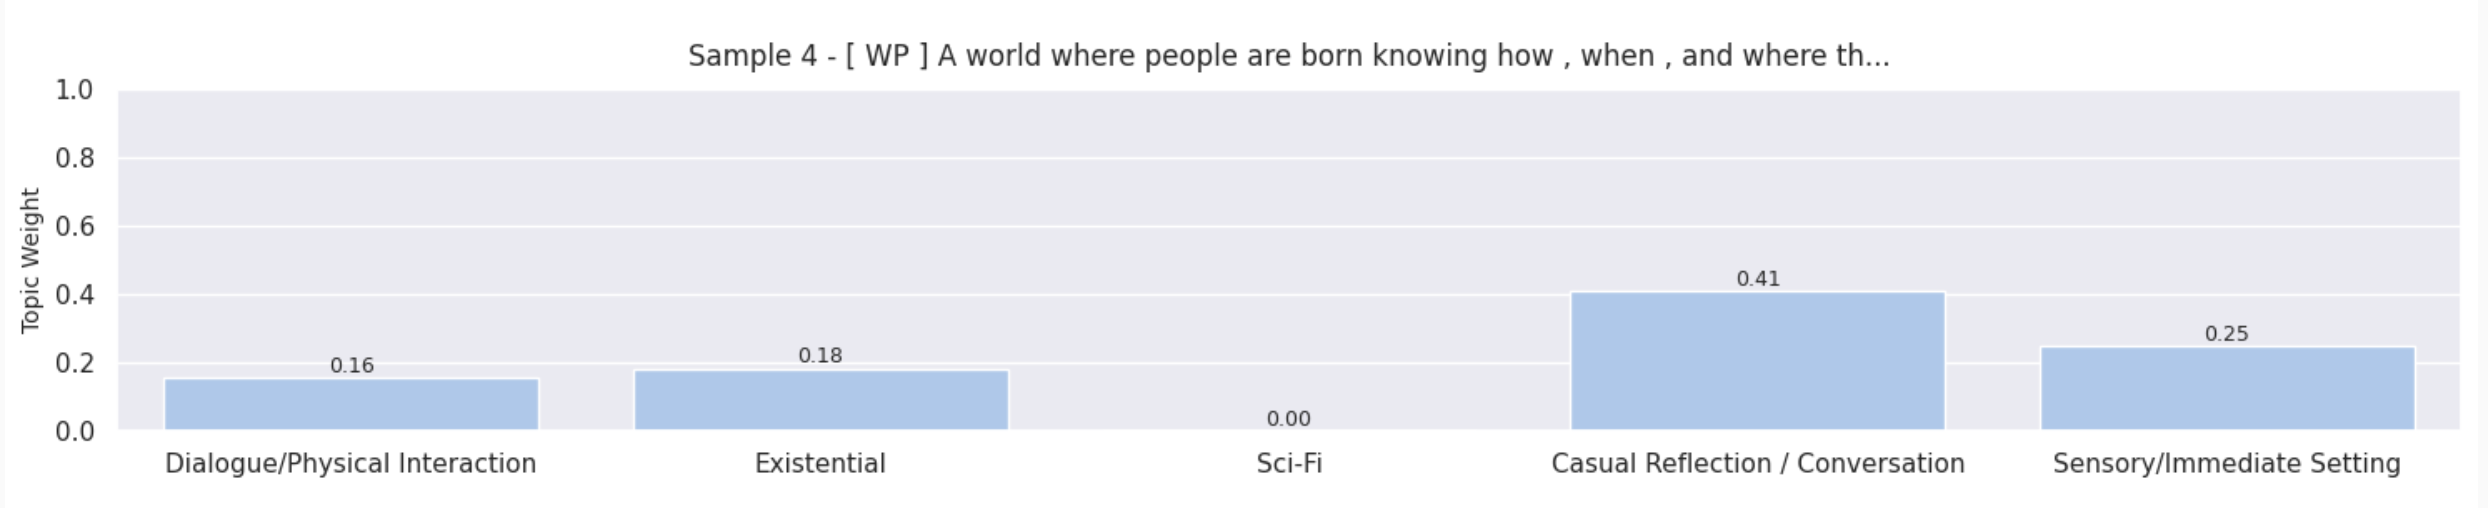
\includegraphics[width=0.5\textwidth]{lda2.png}
    \caption{Plot showing the topic distribution of the given prompt}
    \label{fig:lda2}
\end{figure}

Figures \ref{fig:lda1} and \ref{fig:lda2} are two examples which show the LDA topic distribution for two different prompts.


\section{Text Generation Models}
\subsection{Dataset Preparation}
The dataset was reduced for fine-tuing into 10,000 writing prompts with corresponding stories, split into training, validation, and test sets. The training set contained 8,000 samples, the validation set had 1,000 samples, and the test set also had 1,000 samples. The split was done to ensure that the models could be trained effectively while also being evaluated on unseen data.

\subsection{Metrics for Evaluation}
This section explains various metrics used to evaluate story continuation and generation tasks, particularly with models like BART and T5. These metrics assess different aspects of the generated text's quality, including its overlap with reference texts, semantic similarity, and length.

\subsubsection{ROUGE Scores}
ROUGE (Recall-Oriented Understudy for Gisting Evaluation) is a set of metrics used for evaluating automatic summarization and machine translation software in natural language processing. It works by comparing an automatically produced summary or translation against a set of reference summaries or translations.

\begin{itemize}
    \item \textbf{ROUGE-1}: Measures the overlap of unigrams between the generated text and the reference text
    \item \textbf{ROUGE-2}: Measures the overlap of bigrams between the generated text and the reference text
    \item \textbf{ROUGE-L}: Measures the longest common subsequence (LCS) between the generated text and the reference text, it is sensitive to sentence-level structure and word order.
    \item \textbf{ROUGE-Lsum}: Calculates the LCS score sentence by sentence and then averages them over the entire summary
\end{itemize}

ROUGE scores are crucial for evaluating how well the generated story segment aligns with a reference continuation or a plausible continuation based on human understanding. Higher ROUGE scores generally indicate a better match in terms of word choice and phrasing.
However, perfect scores are rarely achieved or even desirable, as creative generation can deviate while still being good.

\subsubsection{BERT Scores}
BERTScore leverages the contextual embeddings from BERT (Bidirectional Encoder Representations from Transformers) to compute a similarity score, more specifically, semantic similarity.

\begin{itemize}
    \item \textbf{BERT P (Precision)}: Measures how much of the generated text is semantically similar to the reference text
    \item \textbf{BERT R (Recall)}: Measures how much of the reference text is semantically covered by the generated text
    \item \textbf{BERT F1 (F1-Score)}: The harmonic mean of BERT Precision and BERT Recall to balance both precision and recall, offering a comprehensive measure of semantic similarity
\end{itemize}

BERTScore is particularly important because it goes beyond surface-level word matching. It can capture semantic nuances and assess if the generated text "makes sense" in the context of the story, even if it uses different words than a reference. 
Higher BERT scores (closer to 1.0) are indicative of better semantic similarity.

\subsubsection{Length Ratio}
This metric calculates the ratio of the length of the generated text to the length of the reference text. It can be computed based on the number of words or characters.
It is important for assessing whether the model is generating story continuations that are of an appropriate length. Too short a continuation might indicate a lack of detail or completeness, while too long a continuation might suggest verbosity or irrelevant content.


\subsection{Model 1: BART}
\subsubsection{Architecture}

The BART model is developed by Facebook. It is a sequence-to-sequence model designed for both natural language understanding and generation. It features a standard encoder-decoder Transformer architecture, with a bidirectional encoder similar to BERT for comprehensive input understanding and an autoregressive, left-to-right decoder for generating text token by token. 
A key aspect of BART is its pre-training as a denoising autoencoder. This diverse denoising objective allows BART to develop robust capabilities in both understanding and generating coherent text making it highly versatile for a wide range of NLP tasks after fine-tuning.

For this experiment, we employ the \texttt{facebook/bart-base} variant, which consists of 6 encoder and 6 decoder layers, with a hidden size of 768 and approximately 140M parameters.

\subsubsection{Tokenizer}

BART uses a subword tokenizer based on Byte-Pair Encoding (BPE), consistent with RoBERTa. The tokenizer applies dynamic padding and truncation strategies, ensuring sequences are aligned to a maximum length of 512 tokens.

\subsubsection{Fine-Tuning: Training and Results}

The model was fine-tuned for 3 epochs using a batch size of 4, a learning rate of $5 \times 10^{-5}$, and FP16 mixed-precision training. The \texttt{Seq2SeqTrainer} API from HuggingFace was used, along with a custom compute metrics function for evaluation. 

Tables \ref{tab:losses_bart}, \ref{tab:bertscores_bart}, and \ref{tab:rouge_bart} summarize the training progress at selected steps of 500, 1500, 4500, and 6000.

\begin{table}[h!]
\centering
\caption{Losses and Length Ratio for BART}
\begin{tabular}{|c|c|c|c|}
\hline
\textbf{Step} & \textbf{Train Loss} & \textbf{Val Loss} & \textbf{Len Ratio} \\
\hline
500 & 2.85 & 2.90 & 0.0349 \\
1500 & 3.08 & 2.85 & 0.0415 \\
4500 & 2.79 & 2.81 & 0.0387 \\
6000 & 2.77 & 2.80 & 0.0369 \\
\hline
\end{tabular}
\label{tab:losses_bart}
\end{table}

\begin{table}[h!]
\centering
\caption{BERTscores for BART}
\begin{tabular}{|c|c|c|c|}
\hline
\textbf{Step} & \textbf{BERT P} & \textbf{BERT R} & \textbf{BERT F1} \\
\hline
500 & 0.4832 & 0.2755 & 0.3494 \\
1500 & 0.4957 & 0.2834 & 0.3593 \\
4500 & 0.5091 & 0.2889 & 0.3669 \\
6000 & 0.5135 & 0.2884 & 0.3676 \\
\hline
\end{tabular}
\label{tab:bertscores_bart}
\end{table}

\begin{table}[h!]
\centering
\small 
\setlength{\tabcolsep}{4pt} % Reduces the space between columns
\caption{ROUGE Scores for BART}
\begin{tabular}{|c|c|c|c|c|}
\hline
\textbf{Step} & \textbf{Rouge-1} & \textbf{Rouge-2} & \textbf{Rouge-L} & \textbf{Rouge-Lsum} \\
\hline
500 & 0.0366 & 0.0078 & 0.0301 & 0.0340 \\
1500 & 0.0537 & 0.0105 & 0.0414 & 0.0480 \\
4500 & 0.0494 & 0.0114 & 0.0393 & 0.0452 \\
6000 & 0.0456 & 0.0104 & 0.0367 & 0.0422 \\
\hline
\end{tabular}
\label{tab:rouge_bart}
\end{table}

After 6000 steps, the model achieved a training loss of 2.77 and validation loss of 2.80. The best ROUGE-L score recorded was 0.0414 at step 1500, while the BERTScore F1 peaked at 0.3735 around step 3000.



\subsection{Model 2: T5}

\subsubsection{Architecture}

Text-to-Text Transfer Transformer (T5) model is a Transformer-based neural network architecture developed by Google. Its central innovation is to frame all Natural Language Processing (NLP) tasks as a text-to-text problem where both the input and output are always text strings. T
his unified approach simplifies the model's design and enables simultaneous training across a wide array of tasks. T5-Base employs a standard encoder-decoder Transformer architecture. The encoder processes the input text through a stack of Transformer blocks, each featuring a multi-head self-attention mechanism and a feed-forward neural network to produce a contextualized representation. The decoder then generates the target text word by word, using masked multi-head self-attention, a multi-head encoder-decoder attention mechanism to focus on the encoder's output, and a feed-forward neural network. 
Both encoder and decoder layers incorporate residual connections and layer normalization to aid in training deep networks. 

In our experiments, we use the \texttt{t5-base} variant, which includes 12 encoder and 12 decoder layers with a model size of approximately 220M parameters. Unlike BART, T5 is pre-trained using a span-corruption objective and supports prefix-based task prompting.

\subsubsection{Tokenizer}

T5 uses a SentencePiece tokenizer with a fixed vocabulary size of 32,000. Input sequences are prefixed with task-specific instructions. Padding is applied up to a maximum sequence length of 512 tokens.

\subsubsection{Fine-Tuning: Training and Results}

The model was fine-tuned for 3 epochs with a learning rate of $3 \times 10^{-5}$ and batch size of 4, using the \texttt{Seq2SeqTrainer} from HuggingFace. The training schedule included evaluation every 500 steps.

Tables \ref{tab:losses_t5}, \ref{tab:bertscores_t5}, and \ref{tab:rouge_t5} summarize the training progress at selected steps of 500, 1500, 4500, and 6000.

\begin{table}[h!]
\centering
\caption{Losses and Length Ratio for T5}
\begin{tabular}{@{}lccc@{}}
\toprule
\textbf{Step} & \textbf{Train Loss} & \textbf{Val Loss} & \textbf{Len Ratio} \\
\midrule
500 & 3.94 & 3.70 & 0.0217 \\
1500 & 3.81 & 3.57 & 0.0258 \\
4500 & 5.18 & 4.88 & 0.0598 \\
6000 & 5.15 & 4.88 & 0.0598 \\
\bottomrule
\end{tabular}
\label{tab:losses_t5}
\end{table}

\begin{table}[h!]
\centering
\caption{BERT Scores for T5}
\begin{tabular}{@{}lccc@{}}
\toprule
\textbf{Step} & \textbf{BERT P} & \textbf{BERT R} & \textbf{BERT F1} \\
\midrule
500 & 0.5017 & 0.2661 & 0.3451 \\
1500 & 0.4988 & 0.2535 & 0.3348 \\
4500 & 0.4167 & 0.2715 & 0.3281 \\
6000 & 0.4169 & 0.2716 & 0.3282 \\
\bottomrule
\end{tabular}
\label{tab:bertscores_t5}
\end{table}

\begin{table}[h!]
\centering
\small
\setlength{\tabcolsep}{4pt} % Reduces the space between columns
\caption{ROUGE Scores for T5}
\begin{tabular}{@{}lcccc@{}}
\toprule
\textbf{Step} & \textbf{Rouge-1} & \textbf{Rouge-2} & \textbf{Rouge-L} & \textbf{Rouge-Lsum} \\
\midrule
500 & 0.0281 & 0.0048 & 0.0249 & 0.0249 \\
1500 & 0.0298 & 0.0051 & 0.0274 & 0.0274 \\
4500 & 0.0468 & 0.0027 & 0.0405 & 0.0405 \\
6000 & 0.0468 & 0.0027 & 0.0405 & 0.0405 \\
\bottomrule
\end{tabular}
\label{tab:rouge_t5}
\end{table}


By step 6000, T5 achieved a training loss of 5.15 and a validation loss of 4.88. Although BERTScore stabilized around 0.328, ROUGE scores were lower compared to BART.



\section{Comparison and Evaluation}

In this section, we compare the performance of BART and T5 models on the task of story generation / continuation using both zero-shot and fine-tuned setups. The T5 model was prompted with the prefix \texttt{generate story:} in zero-shot and \texttt{Generate a detailed story:} when fine-tuned, while BART was prompted with \texttt{Story:} in fine-tuned case.

\subsection{Zero-Shot Performance}

BART significantly outperforms T5 across all ROUGE and BERTScore metrics with over double the ROUGE-1 and ROUGE-L scores. BART also achieves a higher average length ratio (0.0790 vs. 0.0514), indicating slightly more complete generations. But the results are not satisfactory for either model, as they produce incoherent and contextually irrelevant outputs.
Below are example generations from both models given the same prompt.

\paragraph{Prompt:}
\textit{[EU] Batman snaps, kills the Joker and establishes a reign of terror over Gotham. It's up to Batman's next biggest villains to stop him.}

\paragraph{BART (Zero-Shot) Output:}
\textit{Batman snaps , kills the Joker and establishes a reign of terror over Gotham. It 's up to Batman 's next biggest villans to stop him. "Batman" is out on Blu-ray and DVD on September 14. For more information on the film, go to www.theboxoffice.com.}

\paragraph{T5 (Zero-Shot) Output:}
\textit{Batman snaps , kills the Joker and establishes a reign of terror over Gotham . it 's up to Batman 's next biggest villans to stop him .}

The BART generation contains incomplete and contextually irrelevant text, mostly resembling metadata or titles rather than narrative content. T5's output while more directly aligned with the prompt has barely any difference from the prompt itself. 

These examples illustrate the severe limitations of zero-shot generation for complex, long-form storytelling. Table~\ref{tab:zeroshot-results} summarizes the zero-shot performance of BART and T5 on the story generation task. 

\begin{table}[H]
\centering
\small
\setlength{\tabcolsep}{3pt} % Reduces the space between columns
\caption{Zero-Shot Performance Comparison}
\begin{tabular}{lcc}
\toprule
\textbf{Metric} & \textbf{BART (Zero-Shot)} & \textbf{T5 (Zero-Shot)} \\
\midrule
ROUGE-1 & 0.0980 & 0.0492 \\
ROUGE-2 & 0.0138 & 0.0070 \\
ROUGE-L & 0.0631 & 0.0340 \\
ROUGE-Lsum & 0.0820 & 0.0409 \\
BERTScore Precision & 0.8033 & 0.7757 \\
BERTScore Recall & 0.7692 & 0.7509 \\
BERTScore F1 & 0.7856 & 0.7629 \\
Length Ratio & 0.0790 & 0.0514 \\
\bottomrule
\end{tabular}
\label{tab:zeroshot-results}
\end{table}

\subsection{Fine-Tuned Performance}
Table~\ref{tab:finetuned-results} presents the evaluation of both models after fine-tuning on the task-specific dataset. Fine-tuning leads to substantial improvements across all metrics for both models. 
BART continues to lead in ROUGE and BERTScore metrics. T5 which is still lagging in overall quality scores.

\begin{table}[H]
\centering
\small
\setlength{\tabcolsep}{3pt} % Reduces the space between columns
\caption{Fine-Tuned Performance Comparison}
\begin{tabular}{lcc}
\toprule
\textbf{Metric} & \textbf{BART (Fine-Tuned)} & \textbf{T5 (Fine-Tuned)} \\
\midrule
ROUGE-1 & 0.2871 & 0.1808 \\
ROUGE-2 & 0.0599 & 0.0250 \\
ROUGE-L & 0.1296 & 0.0925 \\
ROUGE-Lsum & 0.2315 & 0.1466 \\
BERTScore Precision & 0.8175 & 0.7552 \\
BERTScore Recall & 0.8054 & 0.7844 \\
BERTScore F1 & 0.8113 & 0.7691 \\
Length Ratio & 0.4787 & 0.4575 \\
\bottomrule
\end{tabular}
\label{tab:finetuned-results}
\end{table}

\subsection{Summary and Comparison}
Overall, BART demonstrates superior performance in both zero-shot and fine-tuned settings for long-form story generation. Fine-tuning significantly enhances the output quality of both models, but BART retains a consistent edge in both lexical and semantic evaluation metrics. T5 is trailing in core scores but provides more diverse lexical outputs. This could be beneficial in generative applications requiring creativity.

\section*{References}

\begin{enumerate}
    \item Lewis, M., Liu, Y., Goyal, N., Ghazvininejad, M., Mohamed, A., Levy, O., ... \& Zettlemoyer, L. (2020).  
    \textit{BART: Denoising Sequence-to-Sequence Pre-training for Natural Language Generation, Translation, and Comprehension}.  
    Proceedings of the 58th Annual Meeting of the Association for Computational Linguistics (ACL), 7871–7880.

    \item Raffel, C., Shazeer, N., Roberts, A., Lee, K., Narang, S., Matena, M., ... \& Liu, P. J. (2020).  
    \textit{Exploring the Limits of Transfer Learning with a Unified Text-to-Text Transformer}.  
    Journal of Machine Learning Research, 21(140), 1–67.

    \item Zhang, T., Kishore, V., Wu, F., Weinberger, K. Q., \& Artzi, Y. (2020).  
    \textit{BERTScore: Evaluating Text Generation with BERT}.  
    International Conference on Learning Representations (ICLR).

    \item Lin, C. Y. (2004).  
    \textit{ROUGE: A Package for Automatic Evaluation of Summaries}.  
    In Text Summarization Branches Out: Proceedings of the ACL-04 Workshop, 74–81.

    \item Wolf, T., Debut, L., Sanh, V., Chaumond, J., Delangue, C., Moi, A., ... \& Rush, A. M. (2020).  
    \textit{Transformers: State-of-the-Art Natural Language Processing}.  
    Proceedings of the 2020 Conference on Empirical Methods in Natural Language Processing: System Demonstrations, 38–45.

    \item Pedregosa, F., Varoquaux, G., Gramfort, A., Michel, V., Thirion, B., Grisel, O., ... \& Duchesnay, É. (2011).  
    \textit{Scikit-learn: Machine Learning in Python}.  
    Journal of Machine Learning Research, 12, 2825–2830.
\end{enumerate}


\end{document}

